% Provenance (never printed): old seconde/premiere S material on the ocean
% (the ocean as a layered fluid, its heat, upwelling and productive waters);
% see sources/book2/PROVENANCE.md. All profiles are WOA23 columns, all
% densities the EOS-80 one-atmosphere equation, computed in
% figdata/grade-10/ocean_profiles.py.
\chapter{The Layered Ocean}\label{ch:g10:layered-ocean}

On a summer day you swim out from a beach into water that is pleasantly warm.
Then you let your legs hang down --- and your feet find water that is
suddenly cold, a couple of metres below the surface. The sea is not mixed
from top to bottom: it is made of layers, warm and light above, cold and
dense below. In the open ocean the same layering reaches down kilometres,
and it decides where the sea is a desert and where it teems with life. This
chapter looks at the ocean in depth: how it is measured, how its temperature
and salinity change downwards, why the layers are stable, and where cold deep
water comes back up to the surface.

\begin{recall}
Seawater contains dissolved salts: its salinity, about 35 grams of salt per
kilogram of seawater on average, varies from sea to sea. Winds drive the
surface currents and the great circular gyres; deep currents of cold, salty
water move slowly along the ocean floor (Book 1, grade 8). Density is mass
divided by volume (the physics books). The phytoplankton, microscopic algae,
need light and mineral nutrients to grow by photosynthesis, and they feed the
rest of the ocean's food chains (the biology books).
\end{recall}

\section{Measuring the ocean}

The ocean covers about \qty{362}{million\ km^2} and is on average
\qty{3682}{m} deep: some \qty{1.33}{billion\ km^3} of water. Most of it lies
far below the reach of light, and it can only be measured by sending
instruments down.
% ledger: charette:ocean-volume

From a ship, oceanographers lower on a cable a frame carrying sensors that
measure the conductivity of the water (from which its salinity is computed),
its temperature and the pressure (hence the depth), surrounded by a ring of
bottles that are closed at chosen depths to bring water samples back on
board. Since the year 2000 a fleet of robotic floats has added millions of
profiles: each float drifts with the currents at a depth of \qty{1000}{m},
sinks every ten days or so to \qty{2000}{m}, then rises to the surface
measuring temperature and salinity on the way, and sends its profile by
satellite.
% ledger: argo:fleet

\begin{dated}{2026}
The international Argo array counts close to 4000 active floats; its
three millionth profile was collected in July 2024.
% ledger: argo:fleet
\end{dated}

\begin{omfigure}
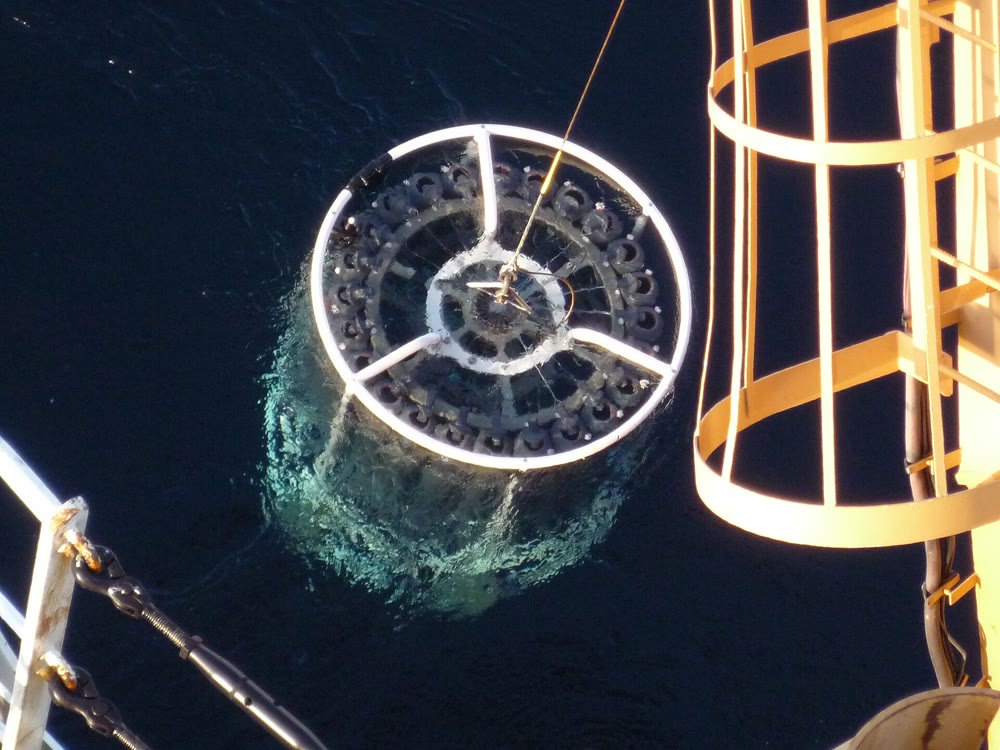
\includegraphics[height=4.4cm]{images/book2/g10-noaa-ctd-rosette.jpg}\hspace{0.4cm}%
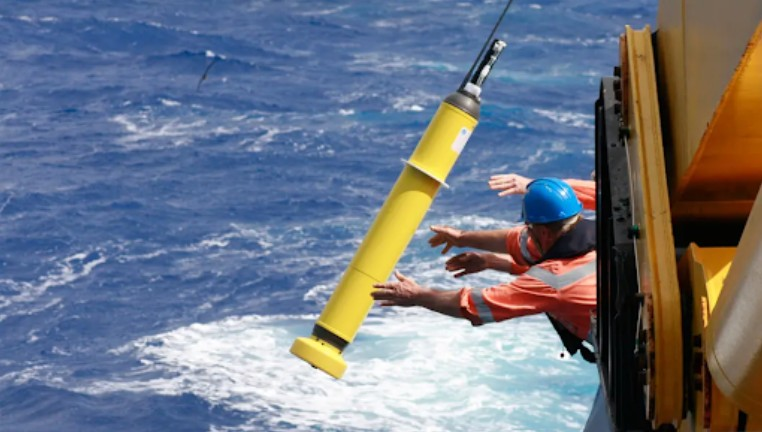
\includegraphics[height=4.4cm]{images/book2/g10-noaa-argo-float.jpg}

{\small Left: a rosette of sampling bottles around its sensors, hauled back
up beside a research ship in the Arctic, 2008 (photograph: Pablo
Clemente-Colon, NOAA Photo Library). Right: a profiling float is launched
from a research ship (photograph: NOAA Global Ocean Monitoring and Observing
Program). Both public domain.}
\end{omfigure}

Averaged over decades of measurements, these profiles give a picture of the
ocean in depth. The profiles of this chapter are such averages, from the
\emph{World Ocean Atlas 2023} of the NOAA National Centers for Environmental
Information.

\section{Temperature with depth}

\begin{omfigure}
\begin{tikzpicture}
\begin{axis}[omrecord, omdepth, width=0.62\linewidth, height=8.2cm,
  axis x line=top, xmin=-3, xmax=31, ymin=0, ymax=2000,
  xlabel={temperature (\unit{\degreeCelsius})}, ylabel={depth (\unit{m})},
  tick label style={font=\small}, label style={font=\small},
  legend style={font=\scriptsize, at={(0.98,0.03)}, anchor=south east}]
\addplot[omThm!85!black, thick] table[x=t, y=depth] {figdata/out/grade-10-ocean_profiles-site-warmpool.dat};
\addplot[omDef!85!black, thick] table[x=t, y=depth] {figdata/out/grade-10-ocean_profiles-site-atlantic.dat};
\addplot[black!70, thick, dashed] table[x=t, y=depth] {figdata/out/grade-10-ocean_profiles-site-arctic.dat};
\legend{{tropical Pacific, 5.5\textdegree N}, {North Atlantic, 40.5\textdegree N}, {Arctic Ocean, 75.5\textdegree N}}
\node[font=\scriptsize, anchor=west] (ml) at (axis cs:21,430) {mixed layer};
\draw[black!50] (ml.north east) -- (axis cs:28.9,35);
\node[font=\scriptsize, anchor=west] (tc) at (axis cs:15.5,600) {thermocline};
\draw[black!50] (tc.north) -- (axis cs:19.9,150);
\node[font=\scriptsize, anchor=west] at (axis cs:7,1500) {deep ocean};
\end{axis}
\end{tikzpicture}

{\small Average temperature against depth at three sites (depth increases
downwards). Data: World Ocean Atlas 2023, annual averages, NOAA NCEI.}
\end{omfigure}
% ledger: data:b2-woa23 (profiles in figdata/grade-10/ocean_profiles.py)

Sunlight heats the ocean from above, in its surface layer. The wind and the waves stir this warm water into a layer of
almost uniform temperature. Below it, the temperature falls quickly over a
few hundred metres; deeper still, it falls slowly to the cold water that
fills the ocean basins.

\begin{definition}[Mixed layer]\label{def:g10:layered-ocean:mixed-layer}
The \emph{mixed layer}\index{mixed layer} is the surface layer of the ocean,
stirred by the wind and the waves, in which temperature and salinity hardly
change with depth.
\end{definition}

\begin{definition}[Thermocline; halocline; pycnocline; deep ocean]\label{def:g10:layered-ocean:thermocline}
The \emph{thermocline}\index{thermocline} is the layer below the \omterm{def:g10:layered-ocean:mixed-layer}{mixed layer} in
which the temperature falls quickly with depth. The layer in which the
salinity changes quickly with depth is a \emph{halocline}\index{halocline};
the layer in which the density increases quickly with depth is the
\emph{pycnocline}\index{pycnocline}. Below them lies the \emph{deep
ocean}\index{deep ocean}, cold and slowly changing.
\end{definition}

In the tropical Pacific the \omterm{def:g10:layered-ocean:mixed-layer}{mixed layer} is at \qty{29.2}{\degreeCelsius} and
some \qty{60}{m} thick; between \qty{70}{m} and \qty{300}{m} the temperature
drops by nearly nineteen degrees, and at \qty{1000}{m} it is down to
\qty{4.5}{\degreeCelsius}. In the North Atlantic the surface is cooler and
the fall more gradual. In the Arctic Ocean the whole column stays within two
degrees of \qty{0}{\degreeCelsius}: there is no warm surface layer to speak
of.
% ledger: data:b2-woa23

\begin{method}[Reading an ocean profile]\label{met:g10:layered-ocean:profile}
\begin{enumerate}
  \item Find the axes: depth increases downwards, the measured quantity is
        read along the top.
  \item The \omterm{def:g10:layered-ocean:mixed-layer}{mixed layer} is the upper part where the curve is nearly
        vertical; its depth is where the curve starts to bend away (a common
        rule: where the temperature has fallen \qty{0.5}{\degreeCelsius}
        below its surface value).
  \item The \omterm{def:g10:layered-ocean:thermocline}{thermocline} is where the curve is closest to horizontal: the
        largest change for the smallest depth.
  \item Below, read the deep values and compare sites at the same depth.
\end{enumerate}
\end{method}

The \omterm{def:g10:layered-ocean:mixed-layer}{mixed layer} changes with the seasons. In winter the surface loses heat,
storms stir the sea, and the \omterm{def:g10:layered-ocean:mixed-layer}{mixed layer} deepens; in summer the sun warms a
thin surface layer that the gentler winds cannot mix downwards, and a
\emph{seasonal \omterm{def:g10:layered-ocean:thermocline}{thermocline}} forms near the surface --- the cold water that
the swimmer's feet find.

\begin{omfigure}
\begin{tikzpicture}
\begin{axis}[omrecord, omdepth, width=0.6\linewidth, height=6.6cm,
  axis x line=top, xmin=12, xmax=24, ymin=0, ymax=300,
  xlabel={temperature (\unit{\degreeCelsius})}, ylabel={depth (\unit{m})},
  tick label style={font=\small}, label style={font=\small},
  legend style={font=\scriptsize, at={(0.98,0.03)}, anchor=south east}]
\addplot[omDef!85!black, thick] table[x=t_feb, y=depth] {figdata/out/grade-10-ocean_profiles-season.dat};
\addplot[omThm!85!black, thick] table[x=t_aug, y=depth] {figdata/out/grade-10-ocean_profiles-season.dat};
\legend{February, August}
\end{axis}
\end{tikzpicture}

{\small Winter and summer in the North Atlantic (40.5\textdegree N,
30.5\textdegree W): monthly average temperatures for February and August.
In February the \omterm{def:g10:layered-ocean:mixed-layer}{mixed layer} reaches about \qty{170}{m}; in August a warm
layer about \qty{15}{m} thick lies on a seasonal \omterm{def:g10:layered-ocean:thermocline}{thermocline}. Data: World
Ocean Atlas 2023, NOAA NCEI.}
\end{omfigure}
% ledger: data:b2-woa23 (mixed-layer depths by the 0.5 degC rule, computed in figdata/grade-10/ocean_profiles.py)

\section{Salinity and density}

The density of seawater depends on its temperature and on its salinity. It
is computed from an internationally agreed formula, the equation of state of
seawater, fitted to laboratory measurements.

\begin{proposition}[Density of seawater]\label{prop:g10:layered-ocean:density}
The density of seawater increases with its salinity and decreases as its
temperature rises. At the pressure of the surface, seawater of salinity 35
has a density of \qty{1028.1}{kg/m^3} at \qty{0}{\degreeCelsius} and
\qty{1023.3}{kg/m^3} at \qty{25}{\degreeCelsius}; pure water at
\qty{4}{\degreeCelsius} has a density of \qty{1000.0}{kg/m^3}.
\end{proposition}
% ledger: unesco:eos80 (values computed in figdata/grade-10/ocean_profiles.py)

\begin{omfigure}
\begin{tikzpicture}
\begin{axis}[omrecord, width=0.7\linewidth, height=6.2cm, xmin=-2, xmax=30,
  ymin=1016, ymax=1033, xlabel={temperature (\unit{\degreeCelsius})},
  ylabel={density (\unit{kg/m^3})}, tick label style={font=\small},
  label style={font=\small}, yticklabel style={/pgf/number format/1000 sep={}}]
\addplot[omThm!85!black, thick] table[x=t, y=rho_s38] {figdata/out/grade-10-ocean_profiles-eos.dat};
\addplot[black!80, thick] table[x=t, y=rho_s35] {figdata/out/grade-10-ocean_profiles-eos.dat};
\addplot[omDef!85!black, thick] table[x=t, y=rho_s30] {figdata/out/grade-10-ocean_profiles-eos.dat};
\node[font=\scriptsize, anchor=south west, omThm!85!black] at (axis cs:1,1030.75) {salinity 38};
\node[font=\scriptsize, anchor=south west] at (axis cs:1,1028.35) {salinity 35};
\node[font=\scriptsize, anchor=south west, omDef!85!black] at (axis cs:1,1024.35) {salinity 30};
\end{axis}
\end{tikzpicture}

{\small The density of seawater at the pressure of the surface, against its
temperature, for three salinities (computed from the international equation
of state of seawater).}
\end{omfigure}
% ledger: unesco:eos80

Two things show on the chart. One unit of salinity adds about
\qty{0.8}{kg/m^3}. One degree of warming removes about \qty{0.31}{kg/m^3}
at \qty{25}{\degreeCelsius}, \qty{0.18}{kg/m^3} at \qty{10}{\degreeCelsius},
but only \qty{0.06}{kg/m^3} near \qty{0}{\degreeCelsius}: in warm seas
temperature controls the density, in cold seas salinity does.
% ledger: unesco:eos80 (slopes computed in figdata/grade-10/ocean_profiles.py)

\begin{remark}
The densities of this chapter are computed at the pressure of the surface.
The pressure of the water above compresses seawater a little, by about
\qty{4}{kg/m^3} per kilometre of depth; oceanographers compare water masses
at the same pressure, so that only temperature and salinity count.
\end{remark}
% ledger: unesco:eos80-checks (computed in figdata/grade-10/ocean_profiles.py: 3.9 kg/m3 per km from the 10000-dbar check values)

\begin{omfigure}
\begin{tikzpicture}
\begin{axis}[name=sal, omrecord, omdepth, width=0.5\linewidth, height=7.2cm,
  axis x line=top, xmin=27.5, xmax=37, ymin=0, ymax=1000,
  xlabel={salinity}, ylabel={depth (\unit{m})},
  tick label style={font=\small}, label style={font=\small}]
\addplot[omThm!85!black, thick] table[x=s, y=depth] {figdata/out/grade-10-ocean_profiles-site-warmpool.dat};
\addplot[omDef!85!black, thick] table[x=s, y=depth] {figdata/out/grade-10-ocean_profiles-site-atlantic.dat};
\addplot[black!70, thick, dashed] table[x=s, y=depth] {figdata/out/grade-10-ocean_profiles-site-arctic.dat};
\node[font=\scriptsize, anchor=west, align=left] at (axis cs:28.2,120) {Arctic\\halocline};
\end{axis}
\begin{axis}[at={(sal.east)}, anchor=west, xshift=0.9cm, omrecord, omdepth,
  width=0.5\linewidth, height=7.2cm, axis x line=top, xmin=1021, xmax=1028.5, yticklabels={},
  ymin=0, ymax=1000, xlabel={density (\unit{kg/m^3})},
  tick label style={font=\small}, label style={font=\small},
  xticklabel style={/pgf/number format/1000 sep={}},
  legend style={font=\scriptsize, at={(0.03,0.03)}, anchor=south west}]
\addplot[omThm!85!black, thick] table[x=rho, y=depth] {figdata/out/grade-10-ocean_profiles-site-warmpool.dat};
\addplot[omDef!85!black, thick] table[x=rho, y=depth] {figdata/out/grade-10-ocean_profiles-site-atlantic.dat};
\addplot[black!70, thick, dashed] table[x=rho, y=depth] {figdata/out/grade-10-ocean_profiles-site-arctic.dat};
\legend{tropical Pacific, North Atlantic, Arctic Ocean}
\end{axis}
\end{tikzpicture}

{\small Salinity (left) and density at the pressure of the surface (right)
against depth, at the three sites of the temperature profiles. At every site
the density increases downwards. Data: World Ocean Atlas 2023, NOAA NCEI;
densities from the international equation of state of seawater.}
\end{omfigure}
% ledger: data:b2-woa23, unesco:eos80

In the tropical Pacific the \omterm{def:g10:layered-ocean:thermocline}{pycnocline} coincides with the \omterm{def:g10:layered-ocean:thermocline}{thermocline}. In the
Arctic Ocean the temperature hardly changes, but the salinity rises from 28
at the surface, freshened by rivers and melting ice, to 34.8 at
\qty{500}{m}: the \omterm{def:g10:layered-ocean:thermocline}{halocline} is the \omterm{def:g10:layered-ocean:thermocline}{pycnocline}. In each case the density
increases downwards.
% ledger: data:b2-woa23

\begin{definition}[Stratification]\label{def:g10:layered-ocean:stratification}
The ocean is \emph{stratified}\index{stratification} when its density
increases with depth: lighter water lies on denser water, in layers.
\end{definition}

A \omterm{def:g10:layered-ocean:stratification}{stratified} ocean is stable. A parcel of water pushed down into denser water
is lighter than its surroundings and floats back up; a parcel pushed up sinks
back. To mix the layers, the wind must work against this, and the stronger
the \omterm{def:g10:layered-ocean:thermocline}{pycnocline}, the harder it is: the \omterm{def:g10:layered-ocean:thermocline}{thermocline} is a lid that separates the
surface from the \omterm{def:g10:layered-ocean:thermocline}{deep ocean}. The \omterm{def:g10:layered-ocean:thermocline}{deep ocean} is filled with water that sank
long ago from the cold polar seas, where surface water becomes dense enough
to sink (Book 1, grade 8).

\section{Upwelling}

\begin{definition}[Upwelling]\label{def:g10:layered-ocean:upwelling}
\emph{Upwelling}\index{upwelling} is the rise of cold water from below the
surface layer, to replace surface water that the wind pushes away. It occurs
along some coasts and in the open ocean.
\end{definition}
% ledger: noaa:upwelling

Along a coast, the wind blowing parallel to the shore drags the surface water;
because of the Earth's rotation the water does not simply follow the wind but
is turned away from it, to the right in the Northern Hemisphere and to the
left in the Southern Hemisphere (how this works is the subject of the
university volumes). Off Peru the wind blows along the shore towards the
equator, and the surface water is pushed out to sea; cold water rises near
the coast to take its place. \omterm{def:g10:layered-ocean:upwelling}{Upwelling} also takes place along the equator,
where the trade winds drive the surface water away from it on both sides.
% ledger: noaa:upwelling, kessler:peru-upwelling

\begin{omfigure}
\begin{tikzpicture}[font=\footnotesize, >={Stealth[length=2mm]}]
  % ocean and thermocline
  \fill[omDef!12] (0,-3.2) rectangle (8.2,0);
  \fill[omDef!30] (0,-3.2) -- (0,-2.0) .. controls (3,-2.0) and (5.5,-1.6) .. (7.4,-0.35) -- (8.2,0) -- (8.2,-3.2) -- cycle;
  \draw[omDef!80!black, dashed] (0,-2.0) .. controls (3,-2.0) and (5.5,-1.6) .. (7.4,-0.35);
  \node[anchor=north west, omDef!80!black] at (0.1,-2.05) {thermocline};
  \node[anchor=west, black!70] at (0.15,-0.9) {warm surface water};
  \node[anchor=west, black!70] at (0.15,-2.75) {cold, nutrient-rich water};
  % land
  \fill[omExo!30, draw=black!60] (7.0,-3.2) -- (8.2,-0.1) -- (8.6,0.0) -- (9.6,1.2) -- (10.6,2.2) -- (10.6,-3.2) -- cycle;
  \node[anchor=south, align=center] at (9.9,-1.6) {land};
  % surface flow and rising water
  \draw[->, thick, omThm!80!black] (7.2,-0.3) -- (3.6,-0.3);
  \node[anchor=south, omThm!80!black] at (5.4,-0.25) {surface water pushed offshore};
  \foreach \x/\y in {6.1/-2.1, 6.8/-1.7} \draw[->, thick, omDef!80!black] (\x,\y) -- (\x+0.45,\y+1.15);
  \node[anchor=north, omDef!80!black, align=center] at (6.0,-2.25) {cold water rises};
  % wind along the shore, northward: with west on the left and east on the
  % right the reader looks north, so the wind goes into the page
  \draw[black!70, thick] (2.6,1.0) circle (0.22);
  \draw[black!70, thick] (2.6,1.0) ++(45:0.22) -- ++(225:0.44) (2.6,1.0) ++(135:0.22) -- ++(315:0.44);
  \node[anchor=west, align=left] at (2.9,1.0) {wind along the shore, towards the equator\\(northward, into the page)};
  \node[anchor=north west, black!60] at (0,-3.25) {$\leftarrow$ west};
  \node[anchor=north east, black!60] at (10.6,-3.25) {east $\rightarrow$};
\end{tikzpicture}

{\small Coastal \omterm{def:g10:layered-ocean:upwelling}{upwelling} off Peru (schematic cross-section from west to
east, not to scale): the wind blows along the shore towards the equator,
northward, into the page; the surface water is turned to its left and pushed out to sea;
cold water from below the \omterm{def:g10:layered-ocean:thermocline}{thermocline} rises near the coast to replace it.}
\end{omfigure}

The water that rises is not only cold. Below the sunlit surface layer, the
remains of dead plankton that sink and decay release the mineral nutrients
that the phytoplankton need. Brought back into the light, these nutrients
make the \omterm{def:g10:layered-ocean:upwelling}{upwelling} regions the most productive waters of the ocean, with the
richest fishing grounds. Where the ocean is strongly \omterm{def:g10:layered-ocean:stratification}{stratified} and nothing
brings deep water up, the sunlit layer runs out of nutrients: the centres of
the subtropical gyres are the deserts of the ocean.
% ledger: noaa:upwelling

\begin{omfigure}
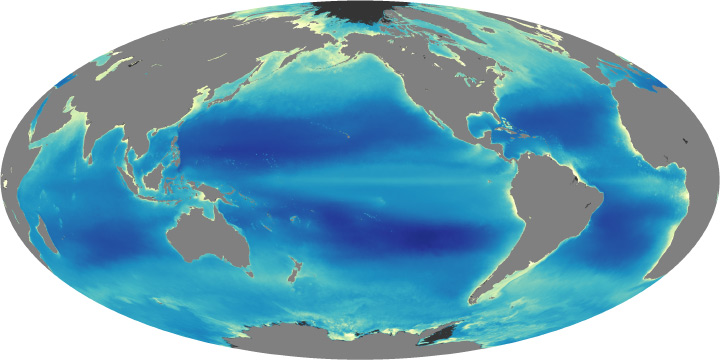
\includegraphics[width=0.8\linewidth]{images/book2/g10-nasa-ocean-chlorophyll.jpg}

{\small The chlorophyll of the phytoplankton seen from space, averaged over
2002--2010: from dark blue (very little) through light blue to yellow (a lot);
land in grey. The coast of Peru and the band along the equator in the
Pacific stand out; the gyres are deep blue. Image: Jesse Allen and Robert
Simmon, NASA Earth Observatory (public domain).}
\end{omfigure}

\begin{omfigure}
\begin{tikzpicture}
\begin{axis}[omrecord, omdepth, width=0.6\linewidth, height=7.2cm,
  axis x line=top, xmin=4, xmax=26, ymin=0, ymax=600,
  xlabel={temperature (\unit{\degreeCelsius})}, ylabel={depth (\unit{m})},
  tick label style={font=\small}, label style={font=\small},
  legend style={font=\scriptsize, at={(0.98,0.03)}, anchor=south east}]
\addplot[omExo!85!black, thick] table[x=t, y=depth] {figdata/out/grade-10-ocean_profiles-site-peru.dat};
\addplot[omThm!85!black, thick] table[x=t, y=depth] {figdata/out/grade-10-ocean_profiles-site-gyre.dat};
\addplot[black!40, dashed, domain=0:600, samples=2] ({15}, {x});
\legend{{off Peru, 13.5\textdegree S}, {South Pacific gyre, 20.5\textdegree S}}
\end{axis}
\end{tikzpicture}

{\small Off Peru, the cold water comes close to the surface: water at
\qty{15}{\degreeCelsius} (dashed line) lies at about \qty{65}{m}, against
nearly \qty{300}{m} in the middle of the South Pacific gyre, which is
farther from the equator. Data: World Ocean Atlas 2023, annual averages,
NOAA NCEI.}
\end{omfigure}
% ledger: data:b2-woa23

\section{Exercises}

\begin{exercise}[$\star$]\label{exo:g10:layered-ocean:1}
Define the \omterm{def:g10:layered-ocean:mixed-layer}{mixed layer} and the \omterm{def:g10:layered-ocean:thermocline}{thermocline}. What stirs the \omterm{def:g10:layered-ocean:mixed-layer}{mixed layer}?
\end{exercise}

\begin{exercise}[$\star$]\label{exo:g10:layered-ocean:2}
Define \omterm{def:g10:layered-ocean:upwelling}{upwelling}. Why are the waters of \omterm{def:g10:layered-ocean:upwelling}{upwelling} regions rich in life?
\end{exercise}

\begin{exercise}[$\star$]\label{exo:g10:layered-ocean:3}
Using the temperature profiles of the three sites, give the temperature at
the surface and at \qty{1000}{m} in the tropical Pacific and in the Arctic
Ocean.
\end{exercise}

\begin{exercise}[$\star$]\label{exo:g10:layered-ocean:4}
Which is denser, seawater of salinity 35 at \qty{25}{\degreeCelsius} or at
\qty{0}{\degreeCelsius}? Seawater of salinity 35 or pure water, at the same
temperature? Use the values of the chapter.
\end{exercise}

\begin{exercise}[$\star$]\label{exo:g10:layered-ocean:5}
Explain how a profiling float measures a profile of the ocean, and why
floats are useful where ships rarely go.
\end{exercise}

\begin{exercise}[$\star\star$]\label{exo:g10:layered-ocean:6}
The ocean covers \qty{361.84}{million\ km^2} with a mean depth of
\qty{3682}{m}. Compute its volume in cubic kilometres. What fraction of its
depth does the top \qty{100}{m} represent?
\end{exercise}

\begin{exercise}[$\star\star$]\label{exo:g10:layered-ocean:7}
In the North Atlantic profile of August, the temperature is
\qty{22.7}{\degreeCelsius} at the surface, \qty{22.2}{\degreeCelsius} at
\qty{15}{m}, \qty{21.8}{\degreeCelsius} at \qty{20}{m} and
\qty{17.3}{\degreeCelsius} at \qty{50}{m}. Using the rule of the method,
estimate the depth of the \omterm{def:g10:layered-ocean:mixed-layer}{mixed layer}. What is the average rate of fall of
temperature between \qty{20}{m} and \qty{50}{m}, in degrees per metre?
\end{exercise}

\begin{exercise}[$\star\star$]\label{exo:g10:layered-ocean:8}
At the same North Atlantic site the surface is at \qty{15.3}{\degreeCelsius}
in February and \qty{22.7}{\degreeCelsius} in August, while at \qty{300}{m}
it is at \qty{13.5}{\degreeCelsius} in both months. Explain why the deep
water does not follow the seasons, and why the winter \omterm{def:g10:layered-ocean:mixed-layer}{mixed layer} is much
deeper than the summer one.
\end{exercise}

\begin{exercise}[$\star\star$]\label{exo:g10:layered-ocean:9}
Near \qty{10}{\degreeCelsius}, one unit of salinity adds
\qty{0.78}{kg/m^3} to the density and one degree of warming removes
\qty{0.18}{kg/m^3}. How many degrees of warming cancel one unit of
salinity? Answer the same question near \qty{0}{\degreeCelsius}, where one
degree removes only \qty{0.06}{kg/m^3}. What do you conclude for the polar
seas?
\end{exercise}

\begin{exercise}[$\star\star$]\label{exo:g10:layered-ocean:10}
In the Arctic Ocean the water at the surface is at \qty{-1.4}{\degreeCelsius}
with a salinity of 28.1, and at \qty{200}{m} at \qty{-1.4}{\degreeCelsius}
with a salinity of 33.3. Their densities are \qty{1022.6}{kg/m^3} and
\qty{1026.8}{kg/m^3}. What makes the deeper water denser? Name the layer
between them.
\end{exercise}

\begin{exercise}[$\star\star$]\label{exo:g10:layered-ocean:11}
Explain why a \omterm{def:g10:layered-ocean:stratification}{stratified} ocean is stable, using a parcel of surface water
pushed down by a wave.
\end{exercise}

\begin{exercise}[$\star\star\star$]\label{exo:g10:layered-ocean:12}
A litre of seawater of salinity 35 at \qty{0}{\degreeCelsius} is warmed to
\qty{25}{\degreeCelsius}. Using the densities of the chapter, compute its
mass, then its new volume. By how much has it expanded, in millilitres? A
layer of ocean \qty{700}{m} thick warms in the same proportion: how much does
its thickness grow? (This is a large exaggeration of real ocean warming,
used here only to show the effect.)
\end{exercise}

\begin{exercise}[$\star\star\star$]\label{exo:g10:layered-ocean:13}
In the tropical Pacific the density is \qty{1021.6}{kg/m^3} at \qty{50}{m}
and \qty{1026.0}{kg/m^3} at \qty{200}{m}; in the North Atlantic in February
the temperature hardly changes over the top \qty{150}{m}. In which of the two
would a storm find it easier to stir the water down to \qty{150}{m}? Explain.
\end{exercise}

\begin{exercise}[$\star\star\star$]\label{exo:g10:layered-ocean:14}
On the chlorophyll map, find two regions of high chlorophyll in the open
ocean far from any coast, and one large region of very low chlorophyll.
Using the chapter, explain each.
\end{exercise}

\begin{exercise}[$\star\star\star$]\label{exo:g10:layered-ocean:15}
Suppose that a float sinks from \qty{1000}{m} to \qty{2000}{m} in six
hours, then rises to the surface in ten hours. Compute its average vertical speed
in each phase, in centimetres per second. If it measured every \qty{2}{s} while
rising, how many measurements does a profile contain, and
what depth separates two of them on average?
\end{exercise}

\section{Problem: A Cast off Peru}

\begin{problem}[{Weekend problem --- two profiles of the South Pacific}]
\label{pb:g10:layered-ocean:1}
% ledger: data:b2-woa23, unesco:eos80 (values rounded from figdata/grade-10/ocean_profiles.py)
The table gives the average temperature and salinity, and the density
computed at the pressure of the surface, at two places of the South Pacific:
off Peru (\qty{13.5}{\degree S}, \qty{77.5}{\degree W}) and in the middle of
the subtropical gyre (\qty{20.5}{\degree S}, \qty{110.5}{\degree W}).

\begin{center}
\small
\begin{tabular}{c|ccc|ccc}
\hline
 & \multicolumn{3}{c|}{off Peru} & \multicolumn{3}{c}{gyre} \\
depth (\unit{m}) & \unit{\degreeCelsius} & salinity & \unit{kg/m^3} & \unit{\degreeCelsius} & salinity & \unit{kg/m^3} \\
\hline
0 & 19.0 & 35.08 & 1025.08 & 24.0 & 36.41 & 1024.71 \\
25 & 17.4 & 35.06 & 1025.47 & 23.9 & 36.39 & 1024.73 \\
50 & 15.8 & 35.03 & 1025.83 & 23.6 & 36.38 & 1024.80 \\
100 & 13.7 & 34.93 & 1026.20 & 22.6 & 36.27 & 1025.02 \\
200 & 12.4 & 34.89 & 1026.44 & 20.3 & 35.80 & 1025.30 \\
300 & 11.1 & 34.80 & 1026.62 & 14.4 & 34.76 & 1025.92 \\
500 & 7.9 & 34.60 & 1026.97 & 7.1 & 34.39 & 1026.92 \\
\hline
\end{tabular}
\end{center}

\medskip
\noindent\textbf{Part I --- Reading the profiles.}
\begin{enumerate}
  \item Which site is warmer at the surface, and by how much?
  \item Which site is farther from the equator? Is the difference of
        surface temperature what you would expect from the latitudes alone?
  \item Using the rule of the method, estimate the depth of the \omterm{def:g10:layered-ocean:mixed-layer}{mixed layer}
        in the gyre.
  \item Is there a \omterm{def:g10:layered-ocean:mixed-layer}{mixed layer} off Peru? Describe the top \qty{100}{m}.
  \item Between which depths does the temperature fall fastest in the gyre?
        Give the rate, in degrees per hundred metres.
  \item At what depth, roughly, is the water at \qty{15}{\degreeCelsius} at
        each site?
\end{enumerate}

\medskip
\noindent\textbf{Part II --- Densities.}
\begin{enumerate}[resume]
  \item Check that the density increases with depth at both sites. What does
        this tell you about their stability?
  \item In the gyre, the surface water is saltier than off Peru. Should this
        make it denser or lighter? Is it denser?
  \item Explain which of the two effects wins.
  \item Compute the increase in density from the surface to \qty{200}{m}
        off Peru.
  \item Compute the same increase in the gyre.
\end{enumerate}

\medskip
\noindent\textbf{Part III --- Stratification compared.}
\begin{enumerate}[resume]
  \item In the gyre, where is most of the density increase of the top
        \qty{500}{m} found: above or below \qty{200}{m}?
  \item Off Peru, where is it found?
  \item At \qty{500}{m}, compare the two sites. What does this suggest about
        the deep water below both?
  \item Explain in a few sentences how the \omterm{def:g10:layered-ocean:thermocline}{thermocline} off Peru has been
        lifted towards the surface.
  \item The phytoplankton live in the top few tens of metres. At which site
        is nutrient-rich water from below the \omterm{def:g10:layered-ocean:thermocline}{thermocline} within reach of the
        wind's stirring? Explain.
\end{enumerate}

\medskip
\noindent\textbf{Part IV --- Why the Peruvian waters are productive.}
\begin{enumerate}[resume]
  \item What would the surface water off Peru be like if the wind along the
        shore stopped blowing for months?
  \item Using the chlorophyll map, compare the two sites.
  \item Explain why the gyre is called a desert of the ocean although it is
        full of sunlight.
  \item Compute the ratio of the density increases from the surface to
        \qty{200}{m} off Peru and in the gyre, and say what it shows.
\end{enumerate}
\end{problem}
